\chapter{Deep Neural Networks}

The history of artificial neural networks (ANN) dates back to 1943. In \cite{McCulloch1943} authors tried to mathematically describe the activity of biological neurons in the human brain. Using these principles they built a first artificial neuron and artificial neural network. In 1974 a PhD student, Paul Werbos, introduced in \cite{Werbos1974} the idea of backpropagation of errors by which ANN are able to learn other than linearly separable problems, and this idea was further expanded in \cite{Rumelhart1986}. Artificial neural networks that contain many hidden layers are also called deep neural networks (DNN) and the process of training this network is called deep learning \cite{LeCun2015}. Over the years deep learning and one of its variants - convolutional neural network that was proposed in \cite{LeCun2015-2} - were found to be very effective and precise in domains that were found unreachable by the classical AI and ML algorithms \cite{LeCun2015}. This was caused by their ability to capture abstract and complex patterns that simpler models found impossible to catch. Such examples include analysis of image data \cite{Farabet2013, Alzubaidi2021} and recent advancements in natural language processing (NLP) \cite{Deng2018}.

\section{Structure}
The fundamental part of every artificial neural network is the neuron. Neuron is basically a function which has one or more inputs and one output. Inside of this neuron, a mathematical computation is being done in order to transform input into output. Input can also be referred to as input vector or vector of input features. Each input feature has its weight by which it is multiplied. Next a bias is added to the multiplied and summed features and weights. This calculation is still linear so in order for it to be able to capture more complex patterns, we need to apply non-linear activation function to its output. The mathematical representation of artificial neuron can be seen in the equation bellow.

\begin{align}
    z &= b + \sum_{i=1}^n (w_i x_i) \\
    a &= f(z)
\end{align}

Where $z$ is the output produced by the linear unit, $b$ is the bias, $n$ is the number of input features, $x_i$ is the \textit{i}-th input feature, $w_i$ is the weight associated with the \textit{i}-th input feature, $a$ is the actual output, and $f$ is the activation function.

Visual example of artificial neuron can be seen in figure \ref{tab:artificial-neuron}.

\begin{figure}[H]
\begin{centering}
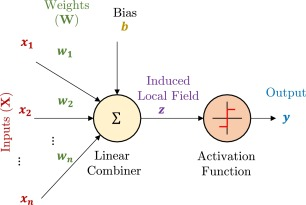
\includegraphics[width=8cm]{assets/images/neuron.jpg}
\par\end{centering}
\caption{Artificial neuron \cite{Santosh2022-1}}
\label{tab:artificial-neuron}
\end{figure}

Similarly to biological neural networks, when artificial neurons are chained together, meaning the output from one neuron is passed to another neuron, they create an artificial neural network.
%TODO: input, hidden, output layer, deep nn, image

\section{Loss Functions}

\section{Training}

\subsection{Forward Propagation}

\subsection{Backpropagation}

\subsection{Hyperparameters}

\section{Evaluation Metrics}

\section{Architectures}